\section{Implementation}
All the flexibility described in the above design criteria is realised by modifying
the headerfiles of my evolvable hardware sourcecode. The implementation was written
in C to ensure efficient execution and quick development cycles. The software can
be cleanly separated into the GUI, the evolution front end, and the FPGA
simulation backend. Collectively they consist of more than 1500 lines of code, with
an extortionate amount of flexibility, capable to scale the size of the FPGA and the
problem well beyond reasonable limits.

\subsection{FPGA Simulation}
The header file for the simulation backend is contained in Appendix~\ref{appx:sim} and shows the
key datastructures and functions exposed to the components performing evolution.
The simulator can convert bitstrings of appropriate length into an FPGA of a
given size, given an FPGA the simulation can also perform evaluations and
simulate faulty logic within any number of cells.

Converting a bitstring to an FPGA is achieved with the function \texttt{bitstring\_to\_fpga},
which takes a pointer to an \texttt{FPGA} struct and a pointer to a char array as arguments.
The cells of the FPGA are iterated over left to right, top to bottom, to fill a shape defined
by \texttt{FPGA\_WIDTH} and \texttt{FPGA\_HEIGHT} and for each cell the next two
bytes are read from the char array. The meaning of the bytes is parsed out and imbedded
in the FPGA struct via an almost direct mapping (north is encoded as 00 in the bitstring,
and is represented as the value 00 in the \texttt{enum} type \texttt{Direction} whenever
a direction is stored on the FPGA).

When evaluating a given input the two values to be operated upon are stored in
the array \texttt{FPGA.input[ FPGA\_WIDTH ]}, then \texttt{evaluate\_fpga} is called.
Each variable and intermediate value
(any value not defining the operation of the FPGA) is intialised to 2 to represent
an undefined value. The simulation then performs a \texttt{tick} step, which iterates over each
cell pulling data from the neighbouring cells, followed by a \texttt{tock} step, which performs
relevent computation and stores output data in relevent output buffers to be read by
the following \texttt{tick} step. These steps continue in turn
until the output is constant (or an iteration cap is reached in which case it halts).
At this point the function returns and the calling entity can inspect cell data and
score accordingly.

The \texttt{tick} step populates each FPGA cells \texttt{n\_in}, \texttt{e\_in},
\texttt{s\_in}, and \texttt{w\_in}, with the relevent data from each neighboring cell.
For example, when assigning \texttt{n\_in} the southern output (\texttt{s\_out})
of the cell to the north is copied in \todo include diagram of this happening.
This occurs for all cells save ones on the edge, if trying
to access a cell beyond the scope of the simulation the variable is assigned the value
representing undefined, 2. This happens uniformly except in the case of the north most cells,
in which cases their \texttt{n\_in} is the relevant value from the \texttt{FPGA.input}
array. Another exception comes of the form of a control signal input; the cell at the top
left is fed a control signal by way of it's \texttt{w\_in} variable, instead of being undefined
it copies the binary value from \texttt{FPGA.control}. This is intended to distinguish
an addition from a subtraction, for an addition the value will be set to either 0 or 1,
and for a subtraction the value will be set to the other, the association has to be
learned by the FPGA configuration during evolution. The way data is made available to an FPGA
is captured by Figure~\ref{fig:control}

\texttt{tock} consults the variables storing information about the operation
performed by the cell, and performs said operation with the relevant $x$\texttt{\_in} variables,
where $x$ represents one of the cardinal direction.
Then each cell's \texttt{n\_out}, \texttt{e\_out}, \texttt{s\_out}, and \texttt{e\_out}
is assigned in accordance with the cells internal mapping (eg. \texttt{n\_out}, the
buffer the cell to the north coppies for it's \texttt{s\_in} value, could be directly
coppied from the function output, or any of the $x$\texttt{\_in} variables).

\todo include diagram for this step too

Deploying this simulation gave subsecond evaluation times for an entire generation of
4x4 FPGAs. These performance benefits, whilst alienating us from the exploitation
of strange undefined behaviour as experienced by Adrian Thompson\cite{10.1007/3-540-63173-9_61}
it did allow considerably quicker software development and the creation of
evolutionary hardware within the strict confines of defined behaviour which
improved the ability to understand the machinations of their success.

\todo a bunch of relevent datastructure diagrams

\subsection{Evolution}
Beyond calls into the simulation backend and inspecting cells after the FPGA
has been evaluated, the evolutionary front end is a distinct entity which operates
almost solely on the abstract bitstrings which constitute the population(s)
being evolved.

\todo talk about datastructures involved, individual, parasite etc. ind has space
for the FPGA struct in it so it doesnt have to be reinstantiated throughout the
process

Initially a population of \texttt{POP\_SIZE} bitstrings of length \texttt{STRING\_LENGTH\_BYTES}
are randomly generated using the pseudorandom \texttt{rand()} syscall, which
(although cryptographically insecure) is suitably random for seeding a random
population. \texttt{STRING\_LENGTH\_BYTES} is defined as \texttt{2 * FPGA\_HEIGHT * FPGA\_WIDTH}.
If \texttt{COEVOLUTION} is defined as \texttt{1} then a population of
parasites of size \texttt{POP\_SIZE}, is also randomly generated. Each parasite
contains an array of size \texttt{PARASITE\_SIZE} containing \texttt{char}s, each of which represents a
challenge posed by the parasite.

The \texttt{evolve} function is passed the randomly seeded population(s) and
curates the evolutionary process. First it randomly seeds an array of potential
faults, these are stored in an array of \texttt{struct}s labeled \texttt{Fault}.
\texttt{Fault} specifies the coordinates of the cell experiencing the fault,
and some auxiliary information depending on the type of fault being simulated.
Whenever an FPGA configuration is created the fault information is coppied into it.
The function then begins on an unending \texttt{while(true)} loop which conducts
the evolutionary process until halted by the user. If coevolving the parasite
population is shuffled and then the each member of the host population is sent
with it's random parasite counterpart to the \texttt{evaluate} step. This function
also requires a pointer to the entire host population. If coevolution is not
happening the function takes a pointer to a dummy parasite instead. When this
function returns the array \texttt{Individual.eval} has been filled. \texttt{eval[0]}
contains the measure of the individuals correctness (already modified by the
weightings given to addition and subtraction), \texttt{eval[1]} denotes the number
of cells on the configuration in the \texttt{OFF} position, and \texttt{eval[2]}
is set to the diversity measurement. While each \texttt{Individual} is
evaluated the mean value for each fitness measurement is collected and the current
most fit individual is kept track of. If coevolving the most fit individual is then
exhaustively tested against all possible input data and the evaluation metrics
are sent to the GUI handler to redraw
the screen. Information about the population fitness, and best case fitness are
logged in an external file. An iteration counter is incremented, the new population(s)
are generated via the \texttt{new\_pop} function and if \texttt{ELITISM}
is defined as \texttt{1} the individual deemed most fit is then coppied directly over
the the 0th element in the new population array.
Then the user input buffer is checked for keyboard input and any relevent
modification made;
'f' activates/deactivates faults, 'd' loads in a perfect adder and assigns highly targeted faults
to act as the fault recovery demonstration, 'r' reseeds the population(s), the
left arrow key shifts the add/sub weightings towards subtraction, and the right
arrow key shifts it towards addition.

\texttt{evaluate} when passed an \texttt{Individual}, a (if not coevolving, dummy) \texttt{Parasite}
and a pointer to the host population populates the evaluation variables in both
the \texttt{Individual} and the \texttt{Parasite}. If not coevolving this is achieved
by first generating the relevent FPGA via the \texttt{bitstring\_to\_fpga} function
and then iterating over all possible inputs, calling \texttt{evaluate\_fpga} and
then reading the required bits from the bottom of the FPGA, one point is given
for each correct bit. This process is completed for both addition and subtraction
and then the weighted average of both is stored in \texttt{Individual.eval[0]}.
Following the evaluation of correctness each cell is iterated over, for every
cell who's function is denoted as \texttt{OFF}, the individual gets 1 point,
and the total is stored in \texttt{Individual.eval[1]}. \texttt{ind\_distance}
gives a measure of the distance between two FPGA configurations, the distance
from the \texttt{Individual} being evaluated and each other individual in the
population is accumulated and the square root mean squared distance is stored
in \texttt{Individual.eval[2]}, this step is an obvious scaling bottleneck but
provides a diversity measurement which vastly improves the chances of successfully
evolving a solution. If coevolving, the set of test additions is defined by the
first half of the \texttt{Parasite} char array, and the set of test subtractions
is defined by the second half of the array. The fitness of an individual is calculated
as before (as the total number of correct output bits) and the parasite score is
given as the maximum score ($bl$ where $b$ is the number of bits checked for each
test, and $l$ is the length of the char array stored in the parasite) minus
the score given to the host individual.

The function \texttt{ind\_distance}
calculates the hamming weight from one FPGA configuration to another. Two
\texttt{Individual}s are passed in and converted into \texttt{FPGA}s via the \texttt{bitstring\_to\_fpga}
function. Then for every
different function and output routing on the configurations, the individuals are 1 further apart.

\texttt{new\_pop} generates a new population of hosts and, if coevolving, parasites.
When coevolving everything done to the host population is mirrored independently
on the parasite population. If using rank-based selection, the population is ordered
based on it's (weighted) fitness; this ordering is conducted via a
population-specific implementation of quicksort. Each population member is associated
a value between $1$ and $n+1$ by the function \texttt{ind\_prob} based on it's ranking
in the population (low fitness individuals have lower rankings), this is the
probability of each individual being selected for the next generation scaled to make
it an integer. Then for each slot in the new population a
random number is generated by \texttt{rand()} between 0 and the sum of all values
generated by \texttt{ind\_prob}.
Starting from zero and the lowest ranked individual, the value given to each population
member is added to the total. If it exceeds the randomly generated number then that
individual is coppied into the open position in the new population. If it does not exceed
the random number the next individual is checked by adding it's value to the running total,
the process is repeated until the random number is exceeded. When all slots in a new
population have been filled the population(s) are mutated. To this end each member is
itterated over and, given an expected mutation rate defined by \texttt{MUTATION} and
genetic material of length $i$, each bit in each individual is flipped with probability
$\frac{1}{i}\texttt{MUTATION}$.

\texttt{ind\_prob} implements Equation~\ref{equ:skew} to skew the ranking to
be more or less discriminatory to highly performing individuals. The skewing
parameter, given as $s$ in the equation is defined by \texttt{PROB\_SKEW} but
this function simply returns it's argument passed through this quadratic equation as
variable $r$.

\todo include graph of selection pressure for different skew values.

In order to store information about the evolutionary process \texttt{log\_data}
writes information about each generation to a \texttt{log.dat} file, which later
can be processed to develop graphs and better understand the quality of the
evolutionary process. The information harvested can be easily modified and
extended but for the most part it has consisted of the mean correctness value
and the correctness of the best case individual.
We are not overly concerned with the total weighted fitness function as we
are using that as a tool to better optimise for correctness; diversity, for
example, is useful for applying evolutionary pressure to preserving a varied
ecosystem but means little for a correct answer and it's effects should be
visible in measuring the correctness alone.

\todo crossover

\todo tournament selection

\todo fancy diagrams

All the evolutionary parameters can be defined at compile time to drastically
alter the execution of the system, all the modifications can be done within
the headerfile \texttt{evolve.h}.

\todo complete function architecture diagram

\subsection{Fault Implimentation}
Faults were implemented by doing a fault pass after each \texttt{tick tock} cycle in
the function \texttt{evaluate\_fgpa} and
overwriting the relevent output of any faulty cells. Before the \texttt{tick} of the
following cycle the predetermined faulty cells have their designated outputs
clamped to a randomly selected value. The fault information is stored in
two arrays within the \texttt{FPGA} struct, the data pertaining to fault
location and effect is stored in an array of type \texttt{Fault}, this has
\texttt{FAULT\_NUM} entries and fully describes the operation of any fault.
A second array of size \texttt{FAULT\_NUM} consisting of integers contains
binary data about whether or not a fault is active on the current evaluation
and controls the execution of the fault pass.

Three types of fault are explored; stuck at 0, stuck at 1, and undefined. In
the first two the result of any logic operation is stuck at a certain value, this
is typical of some sort of short or wearout within a chip. The last type of fault,
undefined faults, always produce a value of 2 (representing undefined) from the function. This means any
output is indiscernible, a value of 2 is always produced by a function if either
of it's inputs are 2s, this models the propagation of uncertainty and a 2 is always
incorrect if read as the answer to a problem from the bottom of the FPGA.

All faults are randomly generated by the \texttt{evolve} function and can be
programmatically activated or deactivated. If the value of \texttt{STICKY} is
set to 1 faults automatically activate/deactivate every 500 generations which
allows for an in depth exploration of the dynamics of evolvable hardware as a
mitigation technique for faults which are sometimes active or sometimes inactive.
This procedure, if allowed to find an always perfect solution, also breeds a solution
which works irrespective of this specific fault. If the fault being modelled is
typical of this hardware this step can be used to develop highly specific
fault tolerant designs.

\subsection{Dynamic Weightings Implimentation}
Programatically or by user input the relative weightings of addition and subtraction
can be shifted mid-execution.

\todo more here

\subsection{GUI}
The user interface is controlled by the simulation backend, which exposes a
series of simple functions to the evolution front end. These exposed functions
allow the triggering of redrawing and reduces the required volume of information
for easy redrawing of the GUI. \texttt{init\_curses} sets up the environment,
\texttt{redraw} called with correct arguments repaints the user interface, and
\texttt{tidy\_up\_curses} cleanly tidies up the GUI.

\begin{figure}
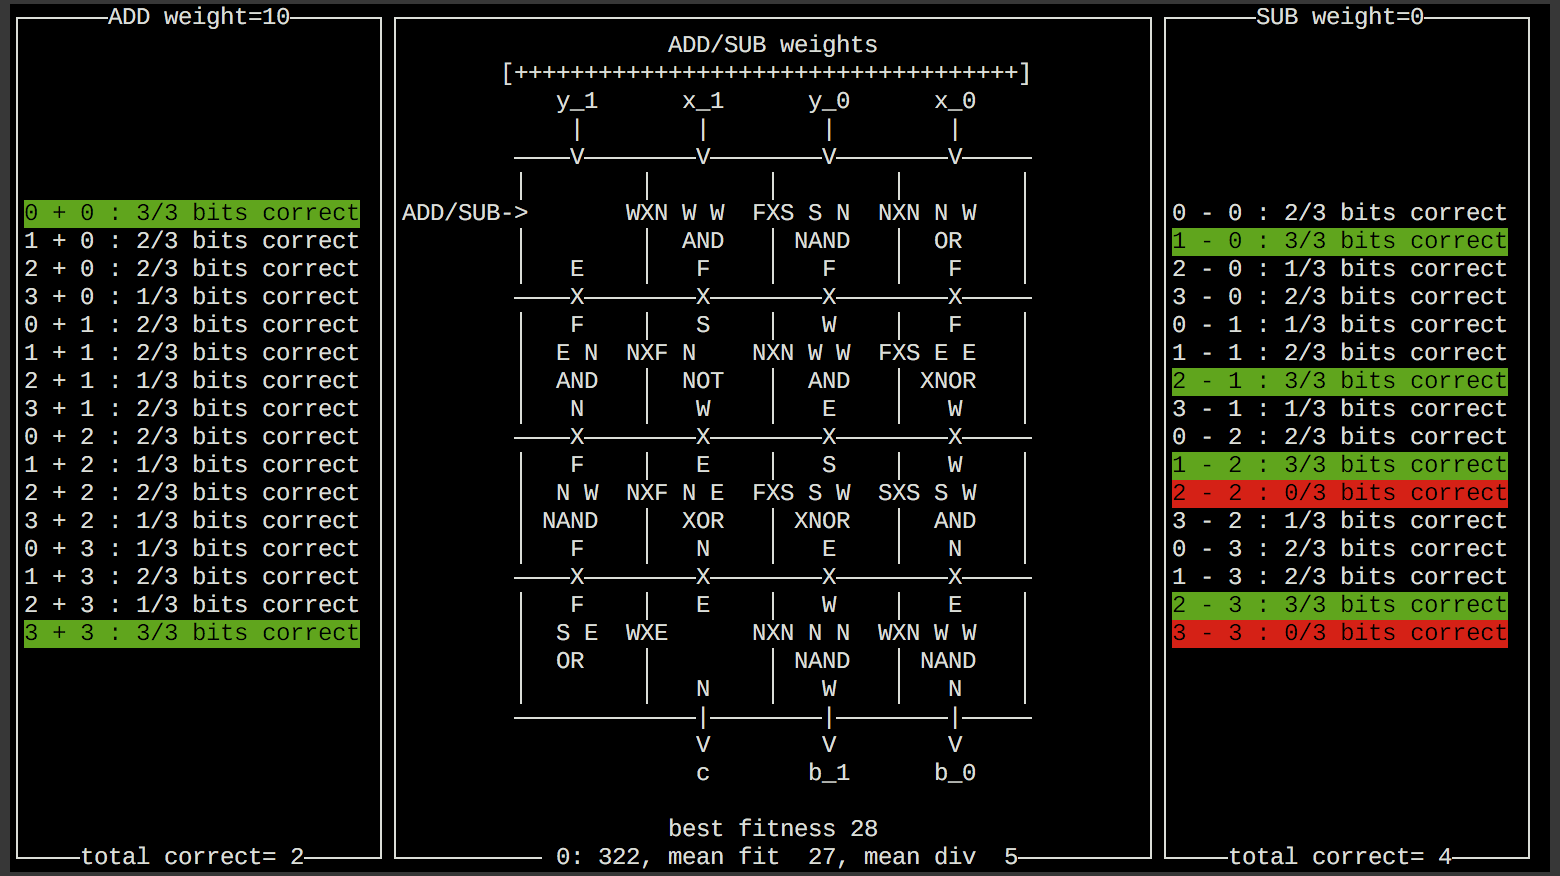
\includegraphics[width=\textwidth]{GUI.png}
\caption{GUI screenshot \todo rescreenshot}
\label{fig:gui}
\end{figure}

The GUI was built with the NCURSES library, a free, open source curses emulation.
It's used to create terminal user interfaces and was chosen due to the amount of
experience  with developing user interfaces with curses, not to
mention a penchant for state-of-the-80s graphics technologies.
Figure~\ref{fig:gui} is a screenshot of the GUI in action. It includes a diagram
of the current best-case FPGA configuration along with it's performance metrics
and information about the underlying population. The panel on the left and right
denote correctly performed addition and subtraction respectively, for a given
if test all 3 bits are correct the test is highlighted in green, if all 3 are wrong
it is highlighted in red.

\todo describe what the gui shows (cell breakdown)

\subsection{Test suite}
The aparatus to perform tests takes the form of a while loop encapsulating the
evolutionary process, reading performance data and meddling with parameters when
required (reseeding the population or changing weightings, for example). The
bounds of the tests being executed are defined in the headerfile \texttt{evolve.h}
(Appendix~\ref{appx:evolve}). \texttt{TEST\_SIZE} defines the number of samples
to be generated, and therefor the number of times the test should be repeated;
\texttt{TEST\_LOOP} defines the size of the inner evolutionary while loop, and
therefore the number of generations each test should be allowed to run for.
During execution information about the best performing individuals, execution time,
and population averages are collected and averaged over each run. This gathered
information is then written to two files \texttt{test.dat}, which involves the
generation-by-generation fitness averages, and \texttt{summary.txt} which details
the number of tests which generated a perfect answer, the average fitness by the
end of execution, and the average execution time.
